% Japanese translation of "Beyond Representation: Index Structure Limitations in Dense Retrieval"
% Compile with: lualatex main_JA.tex  (twice)
% Requires: texlive-langjapanese, adobe-source-han-sans-jp-fonts
\documentclass[conference]{IEEEtran}
\IEEEoverridecommandlockouts

\usepackage{cite}
\usepackage{amsmath,amssymb,amsfonts}
\usepackage{graphicx}
\usepackage{textcomp}
\usepackage{xcolor}
\usepackage{url}
\usepackage{enumitem}
\usepackage{booktabs}

% ---- Japanese (LuaLaTeX-ja) ----
\usepackage{luatexja-fontspec}
\setmainjfont{Source Han Sans JP}
\setsansjfont{Source Han Sans JP}
% -------------------------------

\begin{document}

\title{表現を超えて:密ベクトル検索におけるインデックス構造の限界}

\author{\IEEEauthorblockN{Alessandro Magnani(アレッサンドロ・マニャーニ)}
\IEEEauthorblockA{\textit{独立研究者}\\
ale.magnani@gmail.com}
}

\maketitle

\begin{abstract}
密ベクトル検索(dense retrieval)は,実運用のために HNSW や IVF といった近似最近傍(ANN)インデックスに依存している.これまでの理論研究は主に密埋め込みの\emph{表現}能力に焦点を当ててきたが,本論文ではインデックス化の段階が,それとは別の,定量化可能なボトルネックを生じさせることを示す.我々は\emph{インデックス・バイアス}——厳密検索と近似検索の検索確率の系統的差——を導入し,IDF 重み付きトークンの希少性,埋め込み次元,クラスタ粒度を結びつける「セントロイド希釈上界(centroid-dilution bound)」を導出する.さらに,表現を固定(次元を変えたランダム射影による文字トライグラム埋め込み)し,インデックス構造のみを変化させることで,インデックスに起因する失敗を実証的に切り分ける.評価は Home Depot の商品検索と MS MARCO Passage で行った.加えて,各クエリのセントロイド信号を\emph{直接測定}し,標準クエリから識別子クエリへ移ると信号が約 40 倍崩壊することを観測した.これは理論と観測の間の推論上のギャップを埋めるものである.識別子や希少語に依存する,いわゆる\emph{スピア・フィッシング型}のクエリでは,厳密検索から HNSW 検索に切り替えることで達成可能な Recall@10 の最大 63\% が失われるのに対し,標準的な意味検索クエリではその損失は 2\% 未満である.埋め込み次元を増やすと表現ノイズは低減するが,このインデックス起因のギャップは埋まらない.この結果は「疎か密か」というトレードオフを,表現とインデックスの\emph{同時選択}の問題として捉え直すものであり,部品番号・SKU・固有表現クエリが業務上重要となる本番検索スタックに直接的な示唆を与える.
\end{abstract}

\begin{IEEEkeywords}
密ベクトル検索,近似最近傍探索,インデックス構造,情報検索,サービス品質
\end{IEEEkeywords}

\section{はじめに}
情報検索(IR)は,学習済み埋め込みを用いるニューラルな密ベクトル検索の登場によって大きなパラダイム転換を経験している \cite{ma2022survey}.これは語彙一致に基づく従来の疎検索 \cite{karpukhin2020dense, xiong2021approximate} に対する挑戦である.IR システムは,EC プラットフォームや企業内検索,デジタルアシスタント,ナレッジ管理サービスなど,さまざまなサービス基盤の中核構成要素として使われるようになっており,その信頼性と多様なクエリパターンに対する性能は,ユーザ満足度とサービス品質に直接影響する.

密ベクトル検索では,クエリと文書は連続なベクトル表現に(例えば BERT 系エンコーダで)符号化され,埋め込み空間における最近傍探索によって関連文書が取り出される.このアプローチは意味的理解と結果の適切性を高めることで,多くの情報サービスを刷新してきた.一方,疎検索はテキストを高次元の疎ベクトル(多くは TF-IDF や BM25 の項重み)として表し,重複語を照合するために転置インデックスを用いる.近年では学習済み疎表現も取り入れられている \cite{formal2021splade}.

Tay ら \cite{tay2020sparse} によるランダム射影を用いた理論解析は,十分な次元を持てば密表現は理論上,従来の疎手法と同等またはそれ以上の性能を実現しうることを示唆している.しかしながら,実運用のスケーラビリティは HNSW や IVF などの近似最近傍(ANN)探索アルゴリズムに大きく依存する.埋め込みの表現力については多くの研究がなされてきた一方で,これら不可欠な ANN インデックス構造そのものが課す本質的な限界は比較的未解明のまま残されている.この空白は,多様なユーザ集団による異種のクエリパターンを扱わねばならないシステムを設計するサービスエンジニアにとって,とりわけ深刻な問題となる.

本論文では,ANN インデックス構造が特にいわゆる「スピア・フィッシング」型のクエリ——関連性が希少語や識別子のような特定・非意味的パターンに決定的に依存するクエリ——に対して大きなボトルネックをもたらすことを主張する.これらのクエリは埋め込み空間の疎な領域に位置する文書に対応することが多いが,正確な商品検索や特定情報の照会といった業務上重要なユーザ操作にあたる場合が少なくない.我々は先行研究 \cite{tay2020sparse, fan2022information} を拡張し,一般的な ANN インデックスに内在する近似が,どのようにしてこの種のクエリを系統的に不利にするかを解析する.

本論文の貢献は以下のとおりである.
\begin{itemize}
    \item 「スピア・フィッシング」型クエリの概念を定式化し,標準的な ANN インデックス(IVF と HNSW)が,\emph{表現の理論的能力とは無関係に},これらのクエリで苦戦する理由を理論的に示す.

    \item IDF 重み付きトークン希少性,埋め込み次元 $d$,クラスタリング粒度を結びつける\emph{セントロイド希釈上界}を導出する.これは,IVF のセントロイドが希少トークンの信号を Johnson--Lindenstrauss のノイズ床を上回って保持できない確率に関するものである.さらに,この信号を各クエリで\emph{直接測定}し,Home Depot において標準クエリから ID クエリへ約 40 倍崩壊することを示す.

    \item 3 軸(2 データセット $\times$ 3 クエリタイプ $\times$ 3 埋め込み次元)の制御実験のもと,厳密検索(Flat)と近似検索(IVF・HNSW)を比較することで,インデックス起因の失敗を実証的に切り分け,結果として得られる\emph{インデックス・バイアス}を定量化する.

    \item 上記のギャップが ID クエリと希少語クエリで不釣り合いに大きいこと,また表現の限界とは異なりこのギャップは埋め込み次元を高めても消えないことを示す.
\end{itemize}

\noindent\textit{先行研究に対する新規性.} Tay ら \cite{tay2020sparse} と Fan ら \cite{fan2022information} は密ベクトルの\emph{表現レベル}での能力を解析した.本論文はこれを\emph{インデックスレベル}での解析で補完する.具体的には,表現を(次元を変えたランダム射影の文字トライグラム埋め込みで)固定し,インデックス構造のみを変化させる.これにより観測される劣化はすべてインデックスに帰属できる.第 \ref{sec:theory} 節でこの分離を定式化し,第 \ref{sec:experiments} 節で検証する.

\section{背景と関連研究}

\subsection{密ベクトル検索}
密ベクトル検索モデルは,クエリと文書を連続ベクトル表現に写像する.通常はニューラルネットワークが用いられる.代表例として,クエリと文書に別々の BERT エンコーダを用いる Dense Passage Retriever (DPR) \cite{karpukhin2020dense},表現学習を改善するためにハード負例マイニングを行う ANCE \cite{xiong2021approximate},BERT を意味的類似度比較向けに調整した Sentence-BERT \cite{reimers2019sentencebert} などがある.これらのモデルは関連性ラベル付き大規模データセットで学習され,意味的に関連するクエリと文書を埋め込み空間で近くに配置することを学習する.

より最近では,トークン単位の表現を保持することで細粒度の照合を可能にする ColBERT \cite{khattab2020colbert} のような多ベクトル表現が探究されている.これらは有効である一方,一般に大規模な学習データと計算資源を要する.

\subsection{密表現の理論的能力}
Tay ら \cite{tay2020sparse} は,ランダム射影を用いれば密表現が理論的に疎検索と同等の性能に近づけることを示した.彼らの解析は,十分な次元があれば密ベクトルは疎ベクトルと同じ情報量を捕捉できることを示している.彼らは,これらの理論的洞察と現代的なニューラル構造を組み合わせた潜在ベースの二重エンコーダモデルを導入し,単一ベクトル表現の一部制約を緩和するために多ベクトル表現を提案した.

Fan ら \cite{fan2022information} は密表現の情報理論的解析を行い,クエリのばらつきがどれほど保持されるかを測定した結果,密モデルは疎モデルに比べて分布の裾情報を扱う能力が低いことを示した.この理論的限界は,希少な実体や語彙に対して密検索器が苦戦するという経験的観察を裏付けるものである.

\subsection{密検索のためのインデックス構造}
密ベクトル検索を実用的な規模で運用するには,近似最近傍(ANN)インデックスが不可欠である \cite{johnson2019billion}.実務ではおおむね次の 2 系統が支配的であり,本論文の解析の枠組みも与える.多層の近接グラフを構築し貪欲探索を行う\emph{Hierarchical Navigable Small World}(HNSW)グラフ \cite{malkov2019efficient} と,k-means で文書をクラスタリングし,クエリ時に最も近いセントロイドのみを探る\emph{転置ファイル}(IVF)インデックス(必要に応じて直積量子化 \cite{jegou2010product} と併用)である.どちらも近似によって高速化を達成し,平均的な性能は良いものの,末端(テール)ケースでは系統的に破綻しうる.Lin \cite{lin2024dense} は,HNSW が厳密検索に対して(あまり報告されないものの)わずかに検索品質を落とすことを指摘している.我々は,この小さな\emph{平均}損失が,特定のクエリ集団に集中したはるかに大きな損失を隠していると主張する.

\subsection{研究上の空白}
BEIR \cite{thakur2021beir} のようなベンチマークは,分布外や実体中心のクエリで密検索が失敗することを記録しており,公平性の研究 \cite{zhan2021understanding} も,インデックスレベルの影響が関与していることを示唆している.しかし,ANN インデックス自体の寄与が単独で切り分けられることは稀である.表現の質とインデックス近似の質の相互作用は依然として未解明の課題であり,表現の能力が十分であっても,ANN 探索は不可避的なクエリ単位の失敗様式を生じさせうる.本論文はこのインデックス寄与を構成的に切り分ける.

\section{理論的解析}\label{sec:theory}

我々は密検索のランダム射影的な見方 \cite{tay2020sparse} をインデックス段階へ拡張する.議論は 3 段階からなる:(i) 表現はトークンレベルの信号を持ち,その大きさは IDF 重みと次元に依存する;(ii) 厳密検索は JL 歪みまでこの信号を保存する;(iii) 実用的な ANN 構造は,質的に異なる\emph{第二の}歪みを導入し,希少トークンの信号を不釣り合いに減衰させる.本節における貢献は,セントロイド希釈上界(式 \eqref{eq:centroid_signal_mag}),インデックス・バイアスの分解(式 \eqref{eq:indexing_bias}),そして第 \ref{sec:predictions} 節で述べる 4 つの検証可能な予測(実験が直接検証する)である.

\subsection{設定と信号の大きさ}\label{sec:theory-setup}

Tay ら \cite{tay2020sparse} に倣い,各文書 $d$ を,そのトークン埋め込みの IDF 重み付き和 $f(d)=\sum_{t\in d}\alpha_t\phi(t)$ で表す.ここで $\|\phi(t)\|=1$,$\alpha_t=\log(M/n_t)$,$M$ はコーパスサイズ,$n_t$ は文書頻度である.高次元埋め込み($V$ バケット)は乱数行列 $W$ により次元 $d$ へ射影され,Johnson--Lindenstrauss の補題 \cite{johnson1984extensions} によって内積は乗法的歪み $\epsilon\approx\sqrt{\log V/d}$ の精度で保存される.

\paragraph{希少トークンに対するセントロイド信号.} $N$ 個のクラスタを持つ IVF インデックスにおいて,大きさ $|C|\approx M/N$ のクラスタ $C$ を考える.$p=n_{t^*,C}/|C|$ を希少トークン $t^*$ のクラスタ内出現割合とする.セントロイドは $c=\frac{1}{|C|}\sum_{d\in C}f(d)$ で与えられるので,$c$ には $\alpha_{t^*}\,p\,\phi(t^*)$ の項が含まれる.$t^*$ が支配的なクエリ $q$ の埋め込みはおおよそ $\alpha_{t^*}\phi(t^*)$(正規化を除く)であり,このクエリがそのセントロイドに引き起こすスコアは
\begin{equation}
\langle c, q\rangle \;\approx\; \alpha_{t^*}^2\,p \;=\; \log^2\!\left(\tfrac{M}{n_{t^*}}\right)\cdot\frac{n_{t^*,C}}{M/N}.
\label{eq:centroid_signal_mag}
\end{equation}
IDF が二乗で現れるのは,$\alpha_{t^*}$ がセントロイド側(文書重み経由)とクエリ側の両方に入るためである.これが我々の\emph{セントロイド希釈上界}である:インデックスが少数の大きなクラスタを用いる(小さい $N$)ほど $|C|$ は大きくなり,任意の一つのセントロイドにおける希少トークン信号は縮小する.

\paragraph{信号消失の条件.} JL 射影は内積に大きさ $\epsilon$ のノイズを注入する.希少トークン信号は
\begin{equation}
\alpha_{t^*}^2\,p \;\lesssim\; \epsilon \;\approx\; \sqrt{\tfrac{\log V}{d}}.
\label{eq:signal_loss_general}
\end{equation}
となるとき失われる.$d$ を大きくすると $\epsilon$ は\emph{減少}し,希少トークン検索の助けにはなるが,$\alpha_{t^*}^2 p$ を大きくすることはできない.したがって,$p$ が小さすぎるとき(すなわちクラスタ粒度が粗すぎるとき),次元だけでは検索を救えない.

\subsection{インデックス・バイアス}

$z=Wf(d)$ に対する厳密(Flat)最近傍探索は,これらの内積を JL 歪みまで保存する.ANN 構造はそれとは異なる\emph{第二の}誤差源を持ち込む.これを\emph{インデックス・バイアス}と定義する:
\begin{equation}
\mathrm{Bias}(q,d) \;=\; P_{\text{exact}}(\mathrm{ret}(q,d)) \;-\; P_{\text{approx}}(\mathrm{ret}(q,d)).
\label{eq:indexing_bias}
\end{equation}
IVF ではこれは\emph{クラスタ選択の失敗}として現れる.正しいクラスタが選ばれないのは,そのセントロイドにおける式 \eqref{eq:centroid_signal_mag} の信号がノイズ床を下回るときであり,たとえその中の $t^*$ を含む文書が Flat 検索なら上位に来たとしても選ばれない.HNSW ではこれは\emph{連結性の疎らさ}として現れる.希少トークンに支配される文書の埋め込みは埋め込み空間の低密度領域に位置し,典型的な入口点からの貪欲なグラフ走査ではまず到達されない.いずれの失敗様式も同じクエリ集団——関連性が希少で IDF が高いトークンに依存するもの——を攻撃する.我々はこれらを\emph{スピア・フィッシング型}クエリと呼ぶ.

\subsection{検証可能な予測}\label{sec:predictions}

この枠組みからは,以下の 4 つの実験的に検証可能な予測が導かれる.いずれも第 \ref{sec:experiments} 節の特定の実験に対応している.

\begin{enumerate}
\item \textbf{IVF Recall のスケーリング:} 希少語および ID クエリに対して,IVF Recall@$k$ はプローブ比 ($n_{\text{probes}}/n_{\text{lists}}$) におおむね線形に増加するが,セントロイド希釈により厳密検索の水準には達しない.

\item \textbf{厳密検索と近似検索のギャップ:} 厳密検索と近似検索の性能差は,標準的な意味検索クエリに比べて,希少語・ID クエリで著しく大きい.

\item \textbf{次元の恩恵:} 埋め込み次元 $d$ を大きくすると,射影ノイズ $\epsilon$ が減少するため,ANN 検索下では希少語クエリが不釣り合いに恩恵を受ける.

\item \textbf{インデックス機構の差:} IVF と HNSW はいずれも希少クエリで Flat を下回るが,失敗パターンは機構の違いを反映して異なりうる.
\end{enumerate}

\section{実験}\label{sec:experiments}

我々の実験設計は,表現ファミリを固定してインデックス構造のみを変化させることで,インデックス起因の失敗を切り分ける.具体的には,教師なしの文字トライグラム埋め込みを一定の次元へ射影して用いる.これにより,Flat から ANN への性能低下はすべて,表現ではなくインデックスの効果として解釈できる.

\subsection{セットアップ}\label{sec:setup}

\paragraph{データセットとコーパスの構築.}
対照的なクエリ分布を持つ 2 つのデータセットで評価する:
\begin{itemize}
\item \textbf{Home Depot} (HD): 公開されている Home Depot 商品検索関連性コーパスより.\texttt{product\_uid} で重複を除き $54{,}667$ の一意な商品タイトルを得た.また $11{,}795$ の一意な顧客 \texttt{search\_term} を用い,提供されている「商品 $\to$ クエリ」関連性判定を正解とする.
\item \textbf{MS MARCO Passage v1.1} (MM): \texttt{validation} 分割(10{,}047 クエリ)を用い,各クエリの候補パッセージリストを平坦化して $82{,}360$ のパッセージ文書を得た.\texttt{is\_selected=1} のパッセージを関連文書とする.
\end{itemize}

\paragraph{クエリ部分集合.}
各データセットに対して 3 種類のクエリ部分集合を構成し,それぞれ最大 $1{,}000$ クエリに制限した(該当する場合はシード $42$ で無作為抽出):
\begin{itemize}
\item \textbf{標準 (Standard)}: 提供された関連性判定付きの実ユーザクエリ.
\item \textbf{ID}: 文書識別子を無作為抽出しクエリとしたもの.関連性は自己参照($q{=}d$)とする.この部分集合の索引化時には,識別子文字列を各文書のテキスト先頭に付与する.これは最も極端な「スピア・フィッシング」の状況であり,関連性はただ 1 つの低頻度トークンに依存する.
\item \textbf{希少語 (Rare)}: コーパス中で高々 $5$ 文書にしか出現しないユニグラムまたはバイグラム(アルファベットのみ,長さ $>3$)からなる生成クエリで,そのトークンを含む文書群を関連性集合とする.
\end{itemize}

\paragraph{埋め込みモデル.}
学習済み信号による交絡を避けるため,完全に教師なしの処理系を用いる:\texttt{HashingVectorizer}(バケット数 $2^{18}{=}262{,}144$,文字 $3$-gram(\texttt{analyzer=`char'},\emph{across-token} モード——\texttt{`char\_wb'} でも定性的に同じ傾向であることを確認済み)),に続いて疎な Johnson--Lindenstrauss 射影(\texttt{SparseRandomProjection},密度 $0.9$,シード $42$)で次元 $d\in\{256,512,1024\}$ に落とす.埋め込みは L2 正規化されており,L2 最近傍探索はコサイン類似度探索と等価である.

\paragraph{なぜ「教師なしトライグラム + ランダム射影」がこの研究に\emph{適切な}埋め込みなのか.}
査読者からしばしば挙がる自然な問いは,「なぜ学習済みの密エンコーダ(DPR や Sentence-BERT など)を表現として使わないのか」というものである.答えは方法論的である:本論文の主張は\emph{固定された表現の下でのインデックス}に関するものであり,教師あり学習済みエンコーダは我々の議論が要求する意味で表現を「固定」しえない.トライグラム + JL 射影は L2 距離を既知の乗法歪み $\epsilon\!\propto\!1/\sqrt{d}$ まで保存するので,希少トークン・識別子・SKU の語彙的内容は埋め込みに証明可能な形で残される——これがまさにスピア・フィッシング型クエリの定義そのものである.一方,教師あり意味エンコーダはこれと逆のこと,すなわち語彙的表層形式を捨象することを学習する.5 桁の ID(あるいは表現の乏しい希少ユニグラム)は,それらを引き離すような訓練対がまず存在しないため,埋め込み空間中でほぼ同一の点にマッピングされる.そのようなエンコーダに Flat ベースラインを走らせても,インデックスが結果を歪める前段階で既に識別子クエリで失敗しており,我々が分離しようとしている 2 つの失敗様式を混同することになる.したがって,トライグラムのセットアップは「便宜上のベースライン」ではなく,Flat$\to$ANN のギャップを切り分けるための正しい測定器である.議論の節では,教師ありエンコーダによる確認実験を報告し,スピア・フィッシング型クエリで予測された天井効果的な崩壊が生じることを示す.

\paragraph{検索バックエンドとパラメータ掃引.} すべての密手法は FAISS を用いる:
\begin{itemize}
\item \textbf{Flat}: 全数 L2 探索($P_{\text{exact}}$ ベースライン).
\item \textbf{IVF}: \texttt{IndexIVFFlat},$n_{\text{list}}\in\{200,500,1000\}$ の k-means セル,$n_{\text{probe}}=\lceil n_{\text{list}}\cdot p\rceil$,$p\in\{0.1,0.2,0.5\}$.これにより 1 次元あたり 9 通りの $(n_{\text{list}},n_{\text{probe}})$ 構成となる.
\item \textbf{HNSW}: \texttt{IndexHNSWFlat},$M{=}64$,\texttt{efConstruction}$\in\{100,200\}$,\texttt{efSearch}$=100$.
\item \textbf{BM25}: Pyserini \cite{lin2021pyserini} 経由の Anserini/Lucene(既定パラメータ).
\end{itemize}

\paragraph{評価指標と再現性.}
Recall@$10$ を報告する(Recall@$\{1,5,20,50,100\}$ も計算しており一貫した傾向を確認).全ての数値は各部分集合の $\le 1{,}000$ クエリで集約されている.全掃引(データセットごとに \{部分集合,次元,インデックス,掃引パラメータ\} の直積で $200$ 実行超)はシードにより決定的である.公開コードにより,1 つの JSON 結果ファイルからすべての表と図が生成される.

\subsection{IVF Recall はプローブ比とともに増加するが Flat の下で頭打ちになる}

\begin{figure}[t]
\centerline{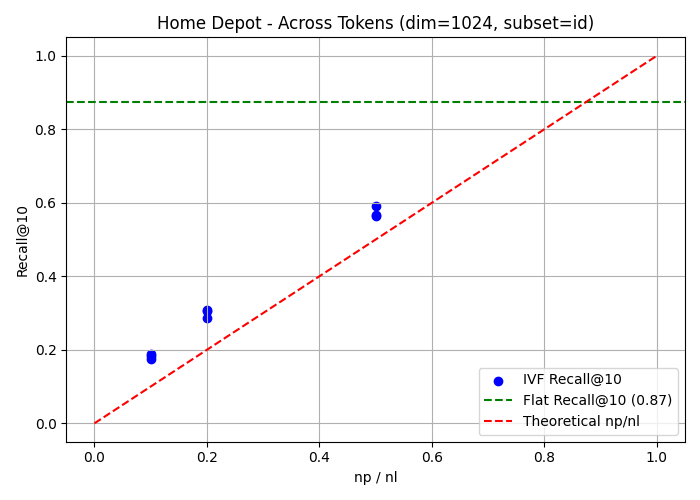
\includegraphics[width=0.49\columnwidth]{figures/home_id_npnl.png}\hfill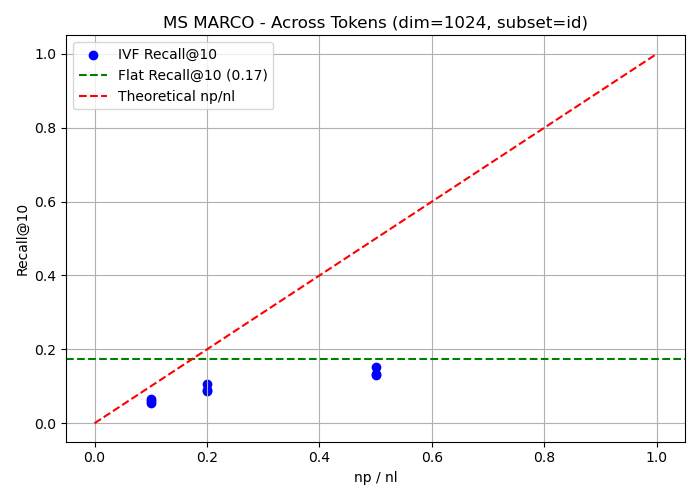
\includegraphics[width=0.49\columnwidth]{figures/msmarco_id_npnl.png}}
\centerline{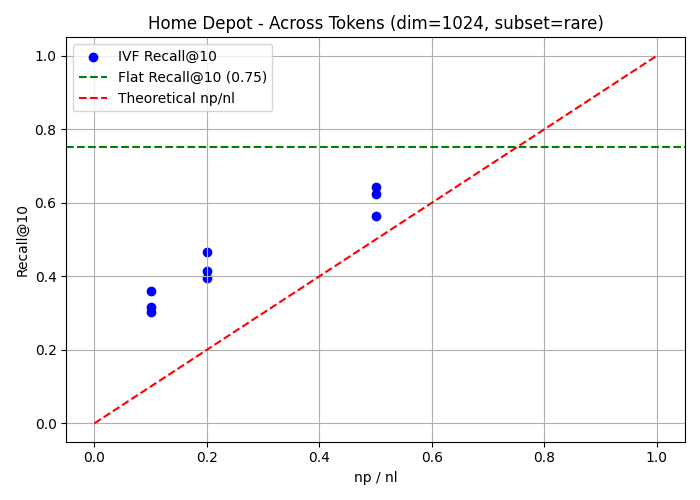
\includegraphics[width=0.49\columnwidth]{figures/home_rare_npnl.png}\hfill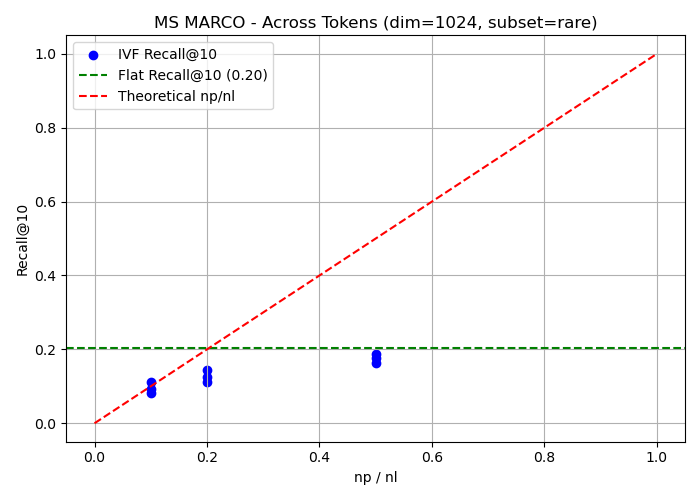
\includegraphics[width=0.49\columnwidth]{figures/msmarco_rare_npnl.png}}
\caption{IVF(青)と Flat(緑破線)の Recall@10 対プローブ比 $n_{\text{probes}}/n_{\text{list}}$,$d{=}1024$.上段:ID クエリ,下段:希少語クエリ.左:Home Depot,右:MS MARCO.どのパネルでも IVF の点群はプローブ比とともに上昇するが Flat には届かない.}
\label{fig:npnl_recall}
\end{figure}

図 \ref{fig:npnl_recall} は\textbf{予測 1} を検証している.IVF Recall@10 は $n_{\text{probes}}/n_{\text{list}}$ に対して単調に(絶対値では劣線形に)上昇する.これは,より広くクラスタを探ることで正しいクラスタを見つけられる頻度が上がるという事実と整合する.しかしプローブ比 $0.5$ に達しても Flat の水準には遠く及ばない.この持続的なギャップは\textbf{予測 2} を支持する:正しいクラスタが選ばれても,セントロイドにおける希少トークンの信号が閾値を下回っており,かつインデックスは選ばれたセル内で信頼できる再順位付けを行わないため,検索はしばしば失敗する.

\subsection{細かなクラスタリングは希少/ID クエリに対して標準クエリよりも大きく効く}

\begin{figure}[t]
\centerline{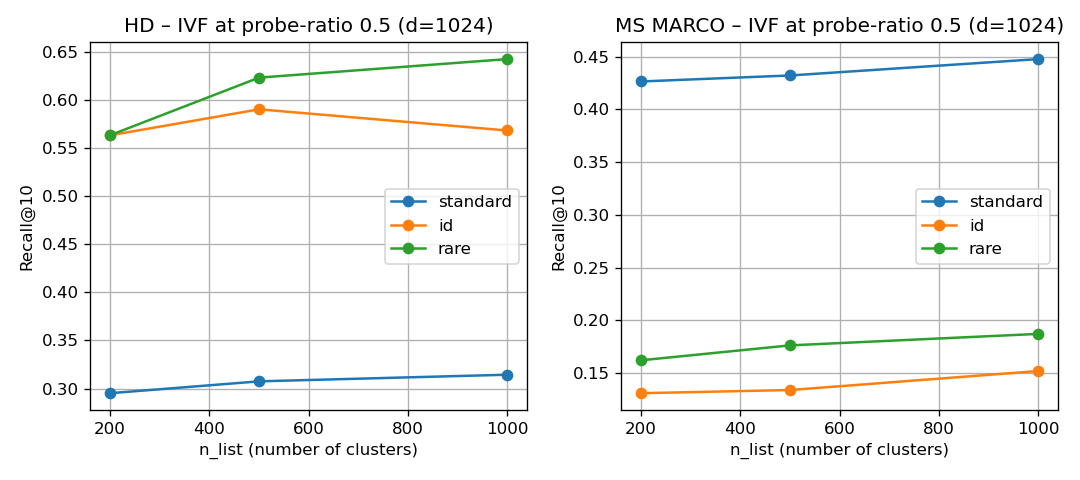
\includegraphics[width=\columnwidth]{figures/ivf_nlist_sensitivity.png}}
\caption{$n_{\text{list}}$ に対する IVF Recall@10(プローブ比 $0.5$,$d{=}1024$).より小さなクラスタ(大きな $n_{\text{list}}$)は\emph{希少語}および\emph{ID}クエリに対して(相対的に)標準クエリの約 2--3 倍恩恵をもたらす.これは式 \eqref{eq:centroid_signal_mag} のセントロイド希釈上界に対する直接的な実証テストである.}
\label{fig:ivf_nlist}
\end{figure}

図 \ref{fig:ivf_nlist} はセントロイド希釈機構の直接的な検証を提供する.式 \eqref{eq:centroid_signal_mag} は,セントロイドあたりの信号の大きさが $N$ に線形に増加(小さい $|C|$ ほどクラスタ内出現割合 $p$ が高い)することを予測している.したがってスピア・フィッシング型クエリは,標準クエリよりも細かなクラスタリングから多くの恩恵を受けるはずである.実際にこの非対称性が観測される:$n_{\text{list}}$ を $200$ から $1000$ に増やすと,希少語クエリの Recall@10 は HD で $+0.079$,MS MARCO で $+0.025$ 向上する(それぞれ相対 14\%,15\%)のに対し,標準クエリでは $+0.019$ と $+0.021$(6\% と 5\%)にとどまる.

\subsection{セントロイド信号の直接測定}\label{sec:dilution-measured}

\begin{figure}[t]
\centerline{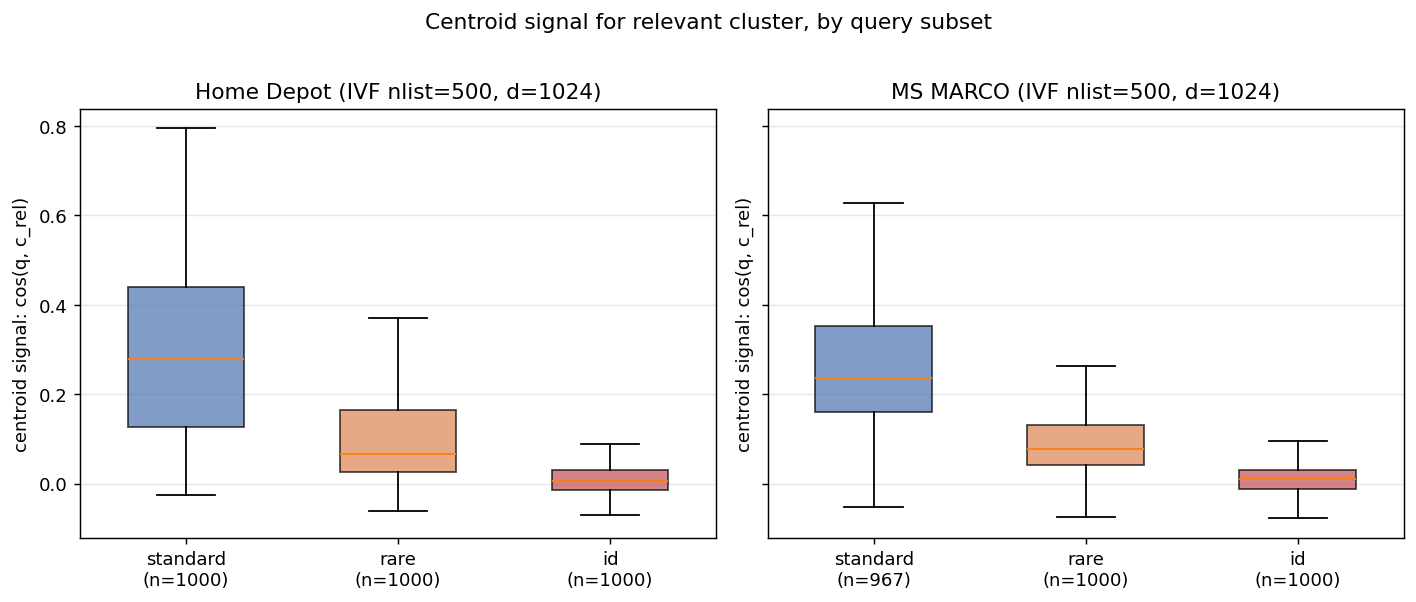
\includegraphics[width=\columnwidth]{figures/centroid_signal_by_subset.png}}
\caption{各クエリの関連クラスタの IVF セントロイド上で測定した,クエリ単位のセントロイド信号 $\langle q, c_{\text{rel}}\rangle$($n_{\text{list}}{=}500$,$d{=}1024$).箱ひげは各部分集合内クエリの分布.Home Depot では,標準から ID にかけて信号の中央値が $\sim\!40$ 倍崩壊する(0.279$\to$0.007).これは式 \eqref{eq:centroid_signal_mag} のセントロイド希釈上界の直接的な実証である.}
\label{fig:centroid_signal}
\end{figure}

集約された Recall@10 からセントロイド希釈を推論するにとどまらず,クエリ単位で直接測定する.各クエリ $q$ について,関連文書を含むクラスタのセントロイド上での信号 $\langle q, c_{\text{rel}}\rangle$ と,そのセントロイドが $500$ 個のセントロイド中で占める\emph{順位}を計算する.表 \ref{tab:centroid-stats} にまとめる.セントロイド信号の中央値は 3 つの部分集合を通じて単調に崩壊する(HD で $0.279\!\to\!0.066\!\to\!0.007$)——$40$ 倍の低下である.探索側からも同じ効果が現れる:関連クラスタは標準クエリの中央値では $2$ 位のセントロイドに対応するが,ID クエリの中央値では($500$ 個中)$216$ 位——下位半分は事実上ランダムと区別できない.プローブ比 $0.5$ において,HD-ID クエリの $41\%$ は\emph{構造的に回復不能}である:正しいクラスタが一度もプローブされないためである.

\begin{table}[t]
\centering
\small
\caption{IVF インデックスにおけるセントロイド希釈の直接測定($n_{\text{list}}{=}500$,$d{=}1024$).Hit@250 は関連クラスタが上位 $250$ 個に入るクエリの割合であり,プローブ比 $0.5$ でプローブされる範囲に対応する.}
\label{tab:centroid-stats}
\setlength{\tabcolsep}{4pt}
\begin{tabular}{llrrr}
\toprule
\textbf{データセット} & \textbf{部分集合} & \textbf{中央値信号} & \textbf{中央値順位} & \textbf{Hit@250} \\
\midrule
HD       & 標準   & 0.279 &   2 & 0.972 \\
HD       & 希少   & 0.066 &  69 & 0.809 \\
HD       & ID     & 0.007 & 216 & 0.591 \\
\midrule
MS MARCO & 標準   & 0.236 &  20 & 0.907 \\
MS MARCO & 希少   & 0.077 & 113 & 0.794 \\
MS MARCO & ID     & 0.011 & 236 & 0.532 \\
\bottomrule
\end{tabular}
\end{table}

\subsection{厳密検索における埋め込み次元}

Flat で $d$ を $256$ から $1024$ に増やすと,HD-ID では Recall@10 が相対で $+74\%$,HD-希少では $+23\%$ 改善するが,HD-標準ではわずか $+16\%$ に過ぎない——これは JL 上界 $\epsilon\!\propto\!1/\sqrt{d}$ と整合する(希少トークンは信号がノイズ床に近く,厚い表現からの恩恵が大きい).ただし,この恩恵は\emph{厳密}検索にのみ及ぶものであり,HNSW を用いると同じ $d{=}1024$ の埋め込みは HD-ID で $0.327$ に停滞する.MS MARCO では,標準・希少語部分集合において Flat 密検索でさえ BM25 を下回る——これは自然言語パッセージに対する教師なし文字トライグラム埋め込みの既知の限界であり,インデックス・バイアスの主張(絶対水準ではなく Flat$\to$ANN のギャップに関するもの)とは独立である.

\subsection{詳細な性能比較}

\begin{table}[t]
\centering
\small
\caption{最良構成での Recall@10}
\label{tab:detailed-results}
\setlength{\tabcolsep}{4pt}
\begin{tabular}{llrrrr}
\toprule
\textbf{データセット} & \textbf{部分集合} & \textbf{Flat} & \textbf{IVF} & \textbf{HNSW} & \textbf{BM25} \\
\midrule
HD       & 標準   & 0.327 & 0.314 & 0.321 & 0.447 \\
HD       & ID     & 0.874 & 0.590 & 0.327 & 1.000 \\
HD       & 希少   & 0.751 & 0.642 & 0.619 & 0.878 \\
\midrule
MS MARCO & 標準   & 0.471 & 0.448 & 0.446 & 0.770 \\
MS MARCO & ID     & 0.174 & 0.152 & 0.071 & 0.000$^{\dagger}$ \\
MS MARCO & 希少   & 0.205 & 0.187 & 0.166 & 0.688 \\
\bottomrule
\end{tabular}
\\[2pt]
{\footnotesize 密検索は $d{=}1024$,across-token トライグラム,最良の ANN 掃引.\\
$^{\dagger}$BM25 は複合的なパッセージ ID をトークン化できない.\\
Flat--HNSW ギャップに関する対応ブートストラップ $95\%$ 信頼区間はすべての行でゼロを含まない.HD-ID: $+0.576$ [$+0.544$, $+0.607$],MM-ID: $+0.138$ [$+0.113$, $+0.162$].}
\end{table}

表 \ref{tab:detailed-results} は $d{=}1024$ における\textbf{予測 2--4} を実証する.

\textbf{予測 2(厳密検索と近似検索のギャップ).} Flat$\to$HNSW のギャップは,スピア・フィッシング型部分集合では標準クエリよりも桁違いに大きい.Home Depot では,このギャップは標準クエリで $0.006$(相対 $1.8\%$),希少クエリで $0.132$($17.5\%$),ID クエリで $0.547$($62.6\%$)である.MS MARCO は絶対 Recall@10 こそ低いが,同じパターンが成り立つ:標準で $0.025$($5.3\%$),希少で $0.039$($19.0\%$),ID で $0.103$($59.2\%$).この「標準対スピア・フィッシング」の対比が本論文の中心的な定量結果である.

\textbf{予測 3(次元).} 埋め込み次元を高くすることは,Flat 検索において,標準クエリよりもスピア・フィッシング型クエリを大きく助ける.HD-ID Flat は $d{=}256$ の $0.501$ から $d{=}1024$ の $0.874$ に伸びる(相対 $74\%$ 増).HD-希少は $0.613 \to 0.751$($23\%$),HD-標準はわずか $0.281 \to 0.327$($16\%$)である.これは JL 上界 $\epsilon\!\approx\!\sqrt{\log V / d}$ と一致する:希少トークンはノイズ床付近に信号を持つため,$\epsilon$ の減少から恩恵を受けやすい.ただし決定的に,次元だけではインデックスのギャップを閉じられない——HD-ID HNSW は $d{=}1024$ でも $0.327$ にとどまる.

\textbf{予測 4(インデックス機構の違い).} IVF は ID クエリで一貫して HNSW を上回る(HD:$0.590$ 対 $0.327$,MM:$0.152$ 対 $0.071$)が,希少および標準部分集合では両者の差は $0.03$ 以内である.これは理論と整合する:ID クエリは極端な連結性失敗の側面を持ち,HNSW の貪欲グラフ走査に IVF の広いクラスタ探索よりも大きな打撃を与える.一方,希少トークン信号はセントロイド希釈(IVF)と連結性喪失(HNSW)を同程度に被る.

\textbf{MS MARCO についての正直な位置づけ.}
MS MARCO の標準・希少部分集合では BM25 が Flat 密検索さえ上回る($0.770$ 対 $0.471$,$0.688$ 対 $0.205$).これは自然言語パッセージに対する教師なしトライグラム埋め込みの表現上の限界であり,本論文が扱う現象ではない.我々の主張は Flat$\to$ANN のギャップに関するものであり,絶対水準に関わらず well-defined である.

\textbf{実用上の可視性(0 件率).}
同じギャップは,ユーザから見える水準——上位 10 件に関連文書を 1 件も返さないクエリの割合——でも顕著に現れる.HD-ID で Flat から HNSW に切り替えると,この割合は $13\%$ から $71\%$ に跳ね上がる.MS MARCO-ID では $78\%$ から $92\%$ である.標準部分集合ではほとんど変化しない(いずれのデータセットでも $\le 2$ パーセントポイント).

\subsection{再現率--レイテンシのトレードオフはスピア・フィッシング型クエリで形が変わる}\label{sec:pareto}

\begin{figure*}[t]
\centering
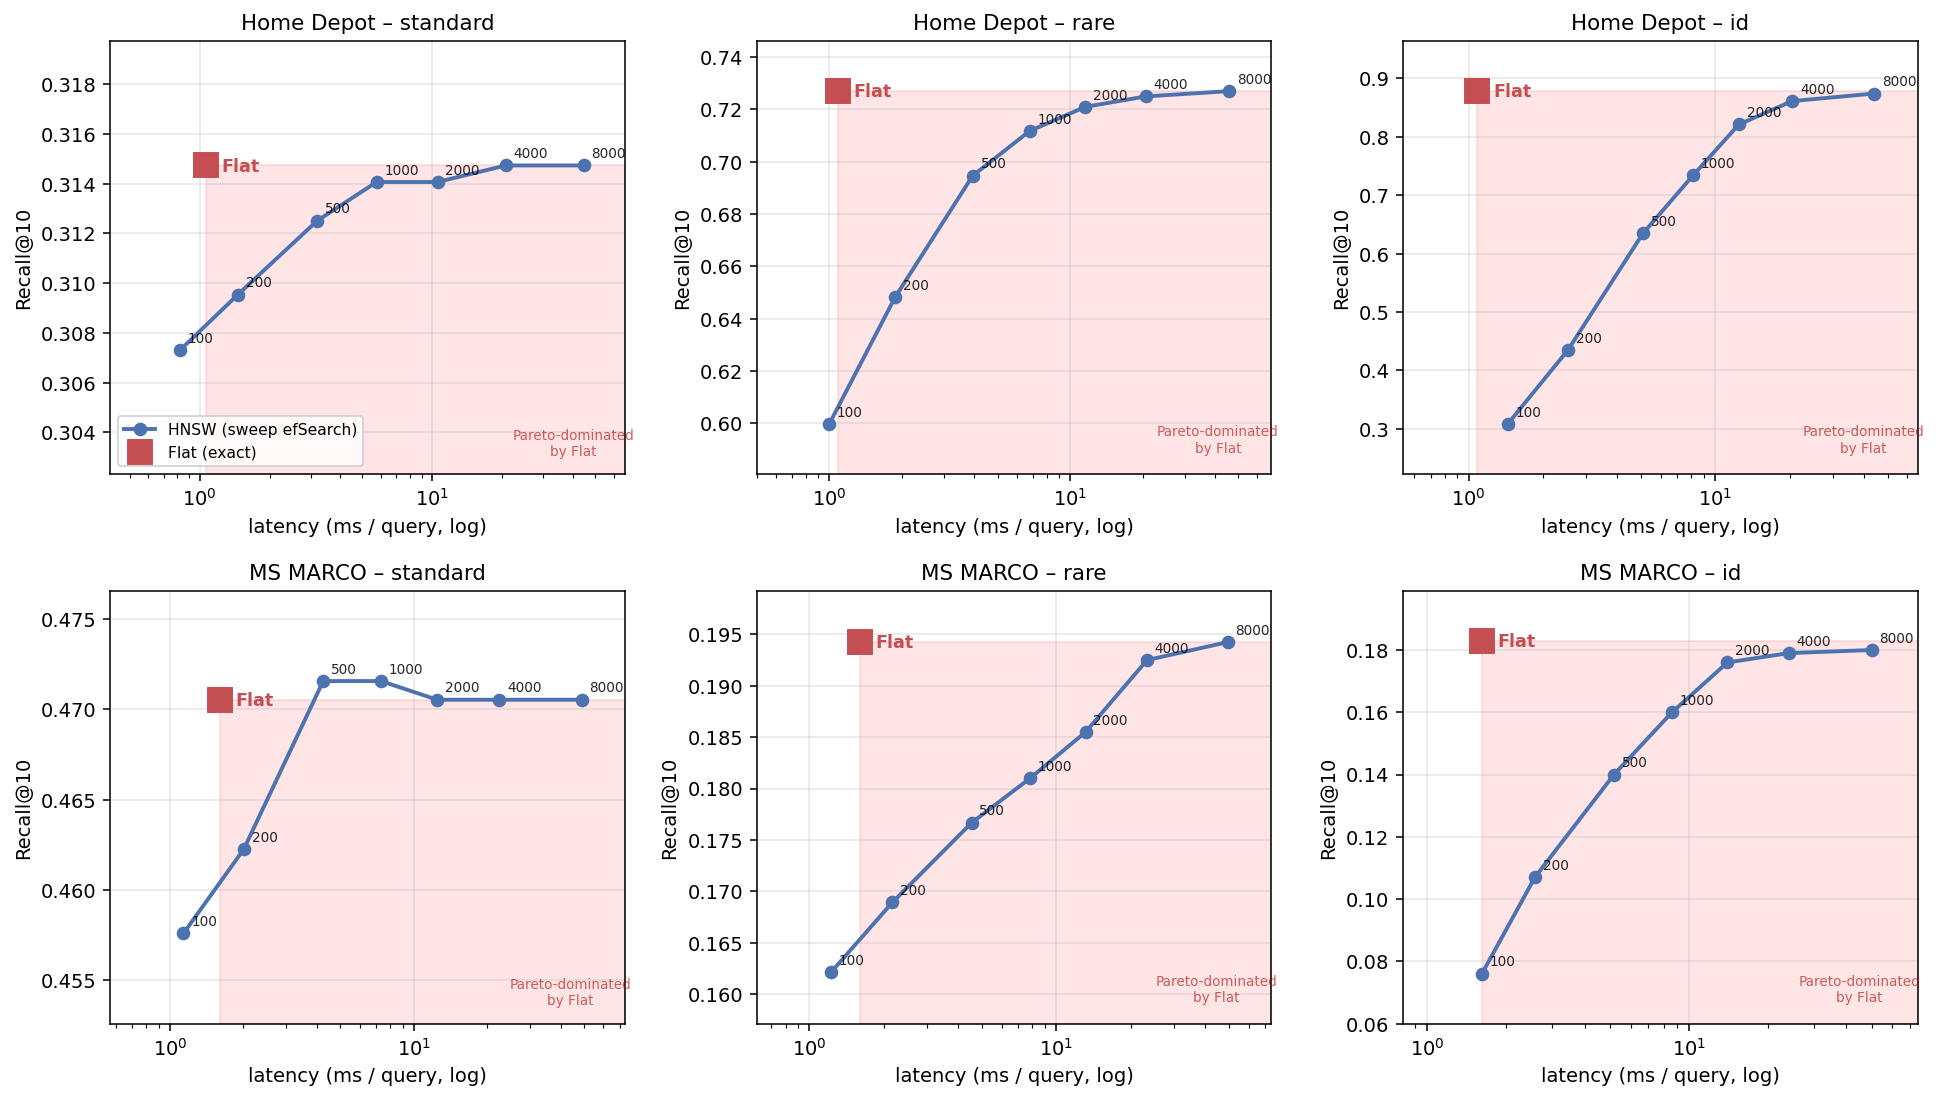
\includegraphics[width=0.95\textwidth]{figures/pareto_recall_vs_latency.png}
\caption{Recall@10 対クエリ単位レイテンシ(x 軸対数),ウォームアップ後の単一スレッド計測.HNSW は標準的な FAISS レシピ $M{=}16$,$\mathrm{efC}{=}200$ で構成し,$\mathrm{efSearch}\in\{50,\dots,16000\}$ を掃引(青曲線,注釈付き).Flat は赤四角一点.赤い陰影域は Flat に厳密に支配される領域(Flat より遅く,かつ再現率も低い)を示す.Flat は構成上再現率の上限を与える.標準部分集合では,HNSW($\mathrm{efS}{=}50$--$100$)は Flat の $2$--$5$ 倍高速で,Flat の再現率の $\ge 92\%$ に到達する——ANN の教科書的なスイートスポット.ID 部分集合では HNSW 曲線の上昇は鈍く,HD-ID は $\mathrm{efS}{=}8000$(Flat のレイテンシの $40\times$)で Flat の $95\%$,MM-ID は $\mathrm{efS}{=}16000$($81\times$)を要する.}
\label{fig:pareto}
\end{figure*}

表 \ref{tab:detailed-results} の Recall@10 は FAISS の既定 \texttt{efSearch}$=100$ における HNSW の値である.完全な描像を得るには \texttt{efSearch} を掃引し,Flat に近づくためのレイテンシコストを測る必要がある.図 \ref{fig:pareto} は標準的な HNSW レシピ $M{=}16$,$\mathrm{efC}{=}200$ で,各(データセット,部分集合)についてこれを示す.HNSW 曲線の形は標準対スピア・フィッシングで質的に異なる.

\paragraph{到達コスト(cost-to-close):コーパス不変な指標.}
図の要約として,Flat の Recall@10 の $95\%$ に到達するのに必要な \texttt{efSearch} と,その結果の Flat に対するレイテンシ比を示す:
\begin{center}\small
\setlength{\tabcolsep}{4pt}
\begin{tabular}{lrrr}
\toprule
部分集合 & Flat の 95\% までの efS & ms/q & Flat との比 \\
\midrule
HD-標準   & $100$    & $0.39$  & $2.7\times$ \emph{高速} \\
HD-希少   & $2{,}000$ & $6.94$  & $6.5\times$ 遅い \\
HD-ID     & $\mathbf{8{,}000}$ & $\mathbf{41.9}$ & $\mathbf{40\times}$ 遅い \\
MM-標準   & $1{,}000$ & $3.48$  & $2.1\times$ 遅い \\
MM-希少   & $16{,}000$ & $129.6$ & $79\times$ 遅い \\
MM-ID     & $\mathbf{16{,}000}$ & $\mathbf{132.0}$ & $\mathbf{81\times}$ 遅い \\
\bottomrule
\end{tabular}
\end{center}
ID クエリのギャップを Flat 再現率の $95\%$ まで閉じるには,同じデータの標準部分集合と比較して $80$--$160\times$ の \texttt{efSearch} 予算が必要となり,本コーパス規模では乗法的に $40$--$80\times$ のレイテンシとなる.コーパス不変な指標はこの \texttt{efSearch} 比そのものである:ANN 探索コストはおおむね \texttt{efSearch} に線形に増えるので,この乗数は任意規模の運用まで持ち越される.

\paragraph{標準クエリ:ANN の教科書的なスイートスポット.}
HD-標準では HNSW efS$=100$ が Flat の再現率の $96\%$ を $0.39$ ms/q で達成する——Flat の $1.07$ ms/q に対して $2.7\times$ 高速.MM-標準では同じ動作点が $82\%$ の再現率を $0.39$ ms/q で達成($4.2\times$ 高速).efS$=50$ では HD-標準は $92\%$ の再現率で $4.7\times$ の高速化を得る.これはまさに HNSW が本番運用向けに設計・利用されている動作点である.

\paragraph{コーパス規模に関する注意.}
我々の $N{\approx}10^5$ では,FAISS Flat は $\sim 1$--$1.6$ ms/q と高速である.密な行列-ベクトル積は SIMD で良く並列化されるためだ.HNSW の対数的高速化の優位はここでは控えめである.$N{=}10^7$ では Flat は線形に遅くなり(${\sim}100$ ms/q),HNSW efS$=100$ は対数的にしか増えないので,\emph{標準}クエリでは HNSW が明確に Flat を凌駕する.一般化するのは\emph{到達コスト比}である:任意の規模において,ID で Flat 級の再現率に到達するには標準の $80$--$160\times$ の \texttt{efSearch} 予算が必要で,HNSW の高速化優位のかなりの部分を消費する.

\subsection{教師ありエンコーダ:方法論の確認実験}\label{sec:supervised-confirm}

セットアップの節では,教師あり意味エンコーダはスピア・フィッシング型クエリを定義する語彙的表層形式を捨象してしまうため,インデックス・バイアス研究のための制御表現には使えない,と理論的に論じた.これを直接検証するため,\texttt{all-MiniLM-L6-v2}(Sentence-BERT,$384$ 次元)で同じグリッドを再走行した.MM-標準ではエンコーダは Flat 再現率をほぼ\emph{倍}にする($0.471 \to 0.894$)——まさにこのエンコーダが学習された領域である.HD-ID では Flat 再現率が $0.874$(トライグラム)から $0.010$(MiniLM)へ\emph{崩壊}し,MM-ID では $0.174$ から $0.001$ へ崩壊する.これらの部分集合では MiniLM 下の Flat$\to$HNSW ギャップは意味を失う.Flat 自体がほぼ何も返さないためである.これは予測した天井効果であり,トライグラム設定が「便宜上のベースライン」ではなく,インデックス段階の失敗を切り分けるために必要な測定器であることを裏付ける.

\section{議論と結論}

我々は\emph{インデックス・バイアス}と\emph{セントロイド希釈上界}を定式化し,4 つの観測可能な結果を予測し,それぞれを確認した:IVF Recall はプローブ比に劣線形にスケールし Flat の下で頭打ちになる;細かなクラスタリングは希少/ID クエリに不釣り合いに効く;クエリ単位のセントロイド信号は標準から ID へ約 40 倍崩壊する(表 \ref{tab:centroid-stats});Flat の再現率の $95\%$ に到達するのに必要な \texttt{efSearch} 予算は ID で標準の $80$--$160$ 倍大きい(図 \ref{fig:pareto})——したがってスピア・フィッシング型ギャップを閉じることは HNSW の速度優位のかなりの部分を消費する.この描像は「疎か密か」の議論を,表現\emph{と}インデックス構造の同時選択の問題として捉え直す:HNSW から得られる標準クエリでの綺麗なトレードオフは,スピア・フィッシング集団に対する急峻な到達コストで支払われている.具体的な今後の方向性は 2 つある:スピア・フィッシング型トラフィックを BM25 または Flat に振り分ける\emph{クエリタイプ意識のルーティング},および,希少特徴の埋め込みを到達困難な領域に置くことにペナルティを与える\emph{インデックス意識の訓練}である.ANN 運用における平均 Recall の報告は,部品番号・SKU・厳密な実体クエリが重要な場面での最悪ケースのサービス品質を大きく過大評価している.

% \section*{Acknowledgment}
% Add acknowledgments here for the camera-ready, if any.

\footnotesize
\begin{thebibliography}{00}

\bibitem{ma2022survey} X. Ma et al., ``A survey on neural information retrieval: At the dawn of the deep learning era,'' ACM Trans. Inf. Syst., vol. 40, no. 2, pp. 1--46, 2022.

\bibitem{karpukhin2020dense} V. Karpukhin et al., ``Dense passage retrieval for open-domain question answering,'' in Proc. Conf. Empirical Methods Natural Language Process., 2020, pp. 6769--6781.

\bibitem{xiong2021approximate} L. Xiong et al., ``Approximate nearest neighbor negative contrastive learning for dense text retrieval,'' in Proc. Int. Conf. Learning Representations, 2021.

\bibitem{formal2021splade} T. Formal et al., ``SPLADE: Sparse lexical and expansion model for first stage ranking,'' in Proc. 44th Int. ACM SIGIR Conf. Research Development Inf. Retrieval, 2021, pp. 2288--2292.

\bibitem{tay2020sparse} Y. Tay, D. Bahri, L. Yang, D. Metzler, and D. C. Juan, ``Sparse splatted array representational learning: A generalization of matrix factorization,'' in Proc. 29th ACM Int. Conf. Inf. Knowledge Manag., 2020, pp. 1425--1434.

\bibitem{fan2022information} Y. Fan et al., ``An information-theoretic analysis of dense retrieval,'' arXiv preprint arXiv:2208.03133, 2022.

\bibitem{lin2024dense} J. Lin, ``A proposed conceptual framework for a representational approach to information retrieval,'' arXiv preprint arXiv:2110.01529, 2024.

\bibitem{reimers2019sentencebert} N. Reimers and I. Gurevych, ``Sentence-BERT: Sentence embeddings using Siamese BERT-networks,'' in Proc. Conf. Empirical Methods Natural Language Process., 2019, pp. 3982--3992.

\bibitem{khattab2020colbert} O. Khattab and M. Zaharia, ``ColBERT: Efficient and effective passage search via contextualized late interaction over BERT,'' in Proc. 43rd Int. ACM SIGIR Conf. Research Development Inf. Retrieval, 2020, pp. 39--48.

\bibitem{johnson2019billion} J. Johnson, M. Douze, and H. Jégou, ``Billion-scale similarity search with GPUs,'' IEEE Trans. Big Data, vol. 7, no. 3, pp. 535--547, 2019.

\bibitem{malkov2019efficient} Y. A. Malkov and D. A. Yashunin, ``Efficient and robust approximate nearest neighbor search using hierarchical navigable small world graphs,'' IEEE Trans. Pattern Anal. Mach. Intell., vol. 42, no. 4, pp. 824--836, 2019.

\bibitem{jegou2010product} H. Jégou, M. Douze, and C. Schmid, ``Product quantization for nearest neighbor search,'' IEEE Trans. Pattern Anal. Mach. Intell., vol. 33, no. 1, pp. 117--128, 2010.

\bibitem{thakur2021beir} N. Thakur et al., ``BEIR: A heterogeneous benchmark for zero-shot evaluation of information retrieval models,'' in Advances in Neural Information Processing Systems, vol. 34, 2021, pp. 9354--9366.

\bibitem{zhan2021understanding} J. Zhan, J. Mao, Y. Liu, M. Zhang, and S. Ma, ``Understanding and improving lexical choice in non-autoregressive translation,'' in Proc. Int. Conf. Learning Representations, 2021.

\bibitem{johnson1984extensions} W. B. Johnson and J. Lindenstrauss, ``Extensions of Lipschitz mappings into a Hilbert space,'' Contemporary Math., vol. 26, pp. 189--206, 1984.

\bibitem{lin2021pyserini} J. Lin et al., ``Pyserini: A Python toolkit for reproducible information retrieval research with sparse and dense representations,'' in Proc. 44th Int. ACM SIGIR Conf. Research Development Inf. Retrieval, 2021, pp. 2356--2362.

\end{thebibliography}

\end{document}
